% Modified for use with Wiley Interdisciplinary Reviews Copyright (C) (2016). All rights reserved.
\documentclass[12pt]{article}

\setlength{\oddsidemargin}{0in}  %left margin position, reference is one inch
\setlength{\textwidth}{6.5in}    %width of text=8.5-1in-1in for margin
\setlength{\topmargin}{-0.5in}    %reference is at 1.5in, -.5in gives a start of about 1in from top
\setlength{\textheight}{9in}     %length of text=11in-1in-1in (top and bot. marg.) 

\usepackage{amsmath,amssymb}
\usepackage{graphicx}% Include figure files
\usepackage{caption}
\usepackage{color}% Include colors for document elements
\usepackage{dcolumn}% Align table columns on decimal point
\usepackage{bm}% bold math
\usepackage{float}
\usepackage{hyperref} % hyperref must be loaded before apacite
\usepackage{apacite}
\bibliographystyle{apacite} 
\hypersetup{ colorlinks = true, citecolor = black, urlcolor = blue}
%\usepackage[nolists, nomarkers, figuresfirst]{endfloat}

\definecolor{background-color}{gray}{0.98}

\title{Place Title Here}
% The title should not exceed 20 words. Please be original and try to include keywords, especially before a colon if applicable, as they will increase the discoverability of your article. Visit http://media.wiley.com/assets/7158/18/SEO_For_Authors.pdf for tips on search engine optimization.

\author{Author A\thanks{Department of Biology, University 1, ...}, Author B\thanks{Department of Chemistry, University 2, ...}, Author C \thanks{Department of Physics, University 3, ...}}
% The preferred (but optional) format for author names is First Name, Middle Initial, Last Name.
% Wiley requires that all authors disclose any potential conflicts of interest.  Any interest or relationship, financial or otherwise, that might be perceived as influencing an author’s objectivity is considered a potential conflict of interest. The existence of a conflict of interest does not preclude publication.

\date{}
\begin{document}
\maketitle

\begin{center}
\subsubsection*{\small Article Type:}
Opinion, Primer, Overview, Advanced Review, Focus Article, or Software Focus
%The Article Type denotes the intended level of readership for your article. An Editor may have mentioned a specific Article Type in your invitation letter; if so, please let them know if you think a different Article Type better suits your topic.

\hfill \break
\thanks

\subsubsection*{Abstract}
\begin{flushleft}
The abstract should not exceed 250 words and should be a concise description of the article and its implications. It should include all keywords associated with your article, as keywords increase its discoverability. Please do not include phrases such as ``This article discusses \ldots" or ``Here we review \ldots", references to other articles, or URLs.
\end{flushleft}
\end{center}


\clearpage

\renewcommand{\baselinestretch}{1.5}
\normalsize

\clearpage

\section*{\sffamily \Large GRAPHICAL TABLE OF CONTENTS} 
Include an attractive full color image for the online Table of Contents. It may be a figure or panel from the article, or may be specifically designed as a visual summary. You will need to upload this as a separate file during submission.

Size: The maximum width and height are 390 pixels, and the minimum resolution is 300 dpi. Multi-panel graphs or images are strongly discouraged.

Caption: This is a narrative sentence to convey the article's essence and wider implications to a non-specialist audience. The maximum length is 50 words, but consider using 140 characters or less to facilitate social media sharing, which can increase the discoverability of your article.

\section*{\sffamily \Large INTRODUCTION} 

Introduce your topic in around 2 paragraphs, around 750 words.  Please define all acronyms at their first usage except IR, UV, NMR, DNA or similar commonly understood terms.  References should use the \href{http://www.apastyle.org/learn/quick-guide-on-references.aspx}{APA style}, like this \cite{coulson1960present}.


\section*{\sffamily \Large First-order heading}
\subsection*{\sffamily \large Second-order heading}
\subsubsection*{\sffamily \normalsize Third-order heading}
Main text paragraphs should be 12 point font, double-spaced, with a maximum of 3 levels of headings (style as shown).

Try to create headings that:
\begin{enumerate}
\item  help the reader find information quickly; 
\item are descriptive yet specific; 
\item are compatible in phrasing and style; and 
\item are concise (less than 50 characters). 
\end{enumerate}

Remember that you are writing for an interdisciplinary audience. Please be sure to discuss interdisciplinary themes, issues, debates, etc. where appropriate. Note that the WIREs are forums for review articles, rather than primary literature describing the results of original research. Reviews should comprehensively survey recent progress in a topic of broad interest, providing the readership with an appreciation of the importance of the work, a summary of recent developments, and a guide to the relevant literature.

\section*{\sffamily \Large EQUATIONS}
Equations should be inserted using standard \LaTeX\ equation and eqnarray environments, not as graphics, and should be set in the main text.
\begin{equation}
\exp (\pi i) = -1
\end{equation}

\section*{\sffamily \Large FIGURES AND TABLES}
Please embed figures and captions in the correct places in the text to facilitate peer review. The [H] next to the figure tag approximately anchors the image to the spot you decide. Production quality figure files are still to be submitted separately. Please note that you will be required to copy the figure captions into the ScholarOne Manuscripts online submission system when uploading your figure files.

Figure captions should stand alone and be informative outside of the context of the article. This will help educators who may want to use a PowerPoint slide of your figure. 

Make sure to include credit lines for any previously published materials. Permission to reuse or adapt previously published materials must be submitted before article acceptance. See \href{http://wires.wiley.com/WileyCDA/Section/id-398153.html#Resources}{here} for more information. See \href{http://media.wiley.com/assets/7315/44/Figure_preparation.pdf}{here} for instructions on figure preparation and formatting.

\begin{figure}[H]
	\centering
	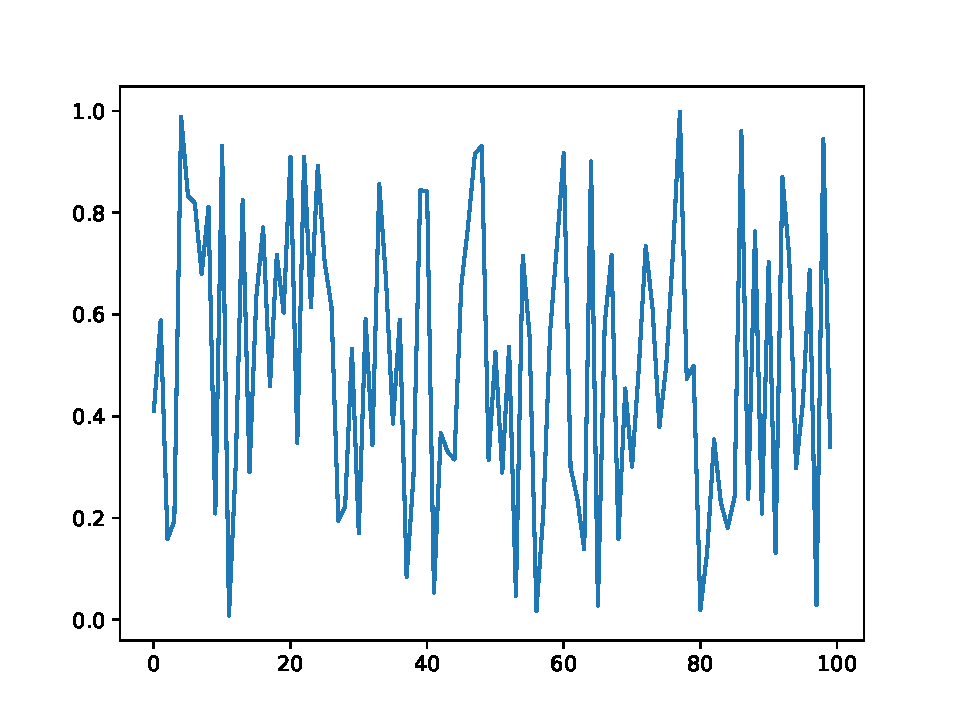
\includegraphics[keepaspectratio=true]{Figure.pdf}
	\caption{Place the figure caption here. In the case of reproduced figures in review articles, you must obtain the publisher's permission and state a suitable notice here along with a citation.  Go \href{http://wires.wiley.com/go/forauthors\#Resources}{here} to get tips on search engine optimization, a guide for designing effective figures, a link to the Copyright Clearance Center for permission requests, and more.}
	\label{fig1} 
\end{figure}

Please include tables in-line in the text by moving the table code to the appropriate place in the text. The [H] approximately anchors the table to the spot you decide.
\begin{table}[H]
	\centering
	\begin{tabular}{|c|c|c|c|}\hline
		\textbf{Quantity} & \textbf{Calculated} & \textbf{Observed} & \textbf{Error} \\ \hline
		Label 1 & n1.1 & n1.2 & Below limit \\ \hline
		Label 2 & n2.1 & n2.2 & Above Limt \\ \hline
	\end{tabular}
	\caption{\label{tbl1} Place table caption here.}
\end{table}






\subsection*{\sffamily \large SIDEBAR}

You are encouraged to include up to two sidebars (“boxed” information that is relevant to but separate from the main text), especially to highlight interdisciplinary themes. Each sidebar should be a maximum of 250 words.

\section*{\sffamily \Large NOTES}
Authors writing from a humanities or social sciences perspective may employ notes as necessary, and only if a comment or additional information is needed to expand on a citation. Notes only containing citations should be converted to references, instead. (Conversely, any references containing comments, such as “For an excellent summary of…,” should be converted to notes.) Notes should be indicated by superscript letters, both in the text and in the notes list. Citations within notes should be listed in the reference section and numbered in order.

\section*{\sffamily \Large ACKNOWLEDGEMENTS}
List contributions from individuals who do not meet the criteria for authorship (for example, to recognize contributions from people who provided technical help, collation of data, writing assistance, acquisition of funding, or a department chairperson who provided general support), with permission from the individual. Financial and material support should also be mentioned. Thanks to anonymous reviewers are not appropriate.


\section*{\sffamily \Large CONCLUSIONS}

Sum up the key conclusions of your review, highlighting the most promising scientific developments, directions for future research, applications, etc. The conclusion should be around 2 paragraphs, around 750 words total.

\section*{\sffamily \Large REFERENCE STYLE}
  Please use the \href{http://www.apastyle.org/learn/quick-guide-on-references.aspx}{APA style} for formatting references.  We have included some references below as an example.

%%%%%%%%%%%%%%%%%%%%%%%%%%%%%%%%%%%%%%%%%%%%%%%%%%%%%%%%%%%%%%%%%%%%%%%%%%%%%%%%%
% BIBLIOGRAPHY

% These should be cited in the text but this is a template so, of course, we don't really reference them. Please include a DOI if available.
\nocite{coulson1960present}
\nocite{hoffmann2008predicting}
\nocite{koros1987separation}
\nocite{malrieu1998quantum}
\nocite{perdew2009some}
\nocite{shaik2007my}
\bibliography{article.bib}

\subsection*{\sffamily \Large FURTHER READING}
%Please insert any further reading/resources here.
For readers who may want more information on concepts in your article, provide full references and/or links to additional recommended resources (books, articles, websites, videos, datasets, etc.) that are not included in the reference section. Please do not include links to non-academic sites, such as Wikipedia, or to impermanent websites.

\end{document}

